\secnumbersection{Ejecución de códigos y análisis de resultados.}
\hlabel{sec:4}

El primer resultado a analizar corresponde a la ejecución del kernel {\verb vectorAdd() } propuesto en el capitulo 3, en ambas tarjetas gráficas utilizadas definiendo un tamaño de vector en aumento.
Los tamaños de vectores utilizado corresponden a una sucesión geométrica definida por la formula,
\begin{equation*}
    M = 2^i , i \in [8,9,\dots,29,30]
\end{equation*}
En la Figura~\ref{fig:16} se presenta el gráfico de tiempo de ejecución (en milisegundos) versus el tamaño del vector.
En este, se puede observar como en las primeras instancias el tiempo de ejecución de la tarjeta de AMD es mucho mayor a la de la tarjeta de NVIDIA.
Sin embargo, para instancias más grandes el tiempo de ejecución se ve disminuido significativamente.
Por otro lado, se nota que la tarjeta de AMD logra ejecutar 2 instancias más para $i = 28$ e $i = 29$, lo cual va de acuerdo a las especificaciones de ambas tarjetas definidas en el capitulo 3.1, presentando una mayor memoria la GPU de AMD.
Esta conclusión se obtiene a partir de la formula de tamaño de memoria teórico de un vector, definido por
\begin{equation}
    m = n \times s
\end{equation}
%$$  s $$
en donde \(m\) corresponde al tamaño total del arreglo en bytes, \(n\) al tamaño del arreglo y \(s\) al tamaño en bytes del elemento utilizado ( 4 en el caso del tipo de dato \textit{float}).
Respecto a la formula anterior, hay que destacar que esta no puede ''igualarse'' a la cantidad de memoria total de la GPU ya que esta también es utilizada por el sistema operativo  para poder renderizar la interfaz de una computadora en al menos aquellas que la utilicen. 

Por último, en lo que concierne a la diferencia de rendimiento en las primeras instancias del gráfico, el principal factor al que se le puede atribuir es a la función de lanzamiento de kernel definido por ROCm ({\verb hipLaunchKernelGGL() }), ya que el otro factor del que podría depender es la inicialización de vectores, pero esto no es considerado en el tiempo de computo de los kernel.

\begin{figure}[h!]
\centering
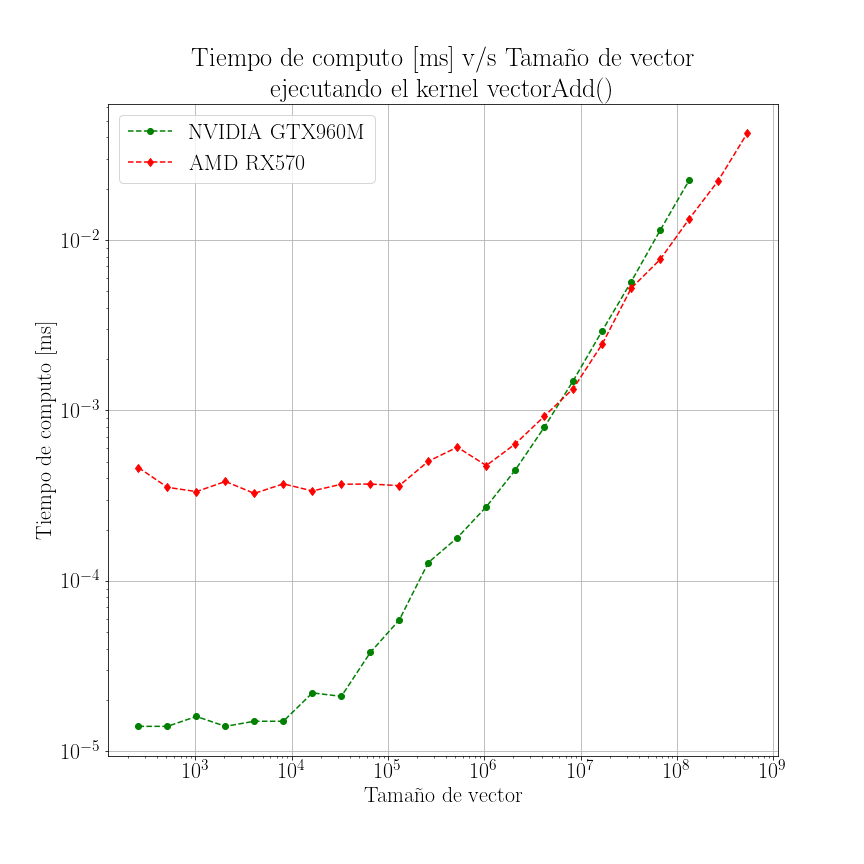
\includegraphics[width=0.8\textwidth]{Figures/plot1.png}
\caption{Gráfico de tiempo de computo versus tamaño de vector al ejecutar el kernel  vectorAdd() .}
\label{fig:16}
\end{figure}

\newpage

%-----------------------------------------------------

El segundo conjunto de resultados, corresponde a la ejecución del kernel {\verb  matrixMul()} en sus cuatro versiones para uso en GPU y explicadas en el Capítulo~\hyperref[sec:3.2]{3.2}, estándar, aplicando \textit{Tiling}, accediendo de forma coalescente en la memoria global y utilizando el producto externo.
Los gráficos de la Figura~\ref{fig:17} corresponden a los resultados (en términos de tiempo de computo y rendimiento) de las distintas versiones de {\verb matrixMul() } antes mencionadas, en ambas tarjetas y para multiplicación de matrices de tamaño \(10240\times10240\), las cuales de acuerdo a la formula 7 utilizan $10240\times10240\times4~\text{[byte]} \approx 419~\text{[Mbyte]}$.
De acuerdo a los resultados, en dos de las tres optimizaciones se observa una mejora significativa respecto a versiones anteriores.
Sin embargo, el acceso coalescente a la memoria global de la matriz de \(B\) provoca en resultados mucho peores que incluso la versión estándar.
Dicho comportamiento puede deberse a un \textit{trade off} entre utilizar un acceso coalescente a la memoria global de \(B\) versus un cambio de forma en el acceso a la memoria compartida, mejor conocido como \textit{Bank Conflict}.
Este termino viene en que, para aumentar el ancho de banda efectivo al realizar accesos a memoria compartida, los datos de esta están divididos en diferentes módulos (o \textit{Banks}).
Así, si múltiples \textit{threads} deben hacer accesos a diferentes \textit{Banks} estos serán simultáneos, mientras que si se deben realizar accesos a un mismo \textit{Bank}, estos se harán de forma secuencial \cite{bank}.

Otra diferencia encontrada es que en la versión de acceso coalescente a memoria global, el resultado de NVIDIA es peor tanto en Gflop/s como en tiempo de ejecución respecto de la versión estándar, mientras que en AMD el resultado sigue siendo un poco mejor.
Esto puede deberse a un manejo optimizado en el acceso a memorias por parte de los controladores de AMD, evidenciando así mismo un mejor rendimiento general para dicho volumen de datos (dejando de lado las especificaciones generales). 

\begin{figure}[H]
  \centering
  \begin{subfigure}{0.5\textwidth}
    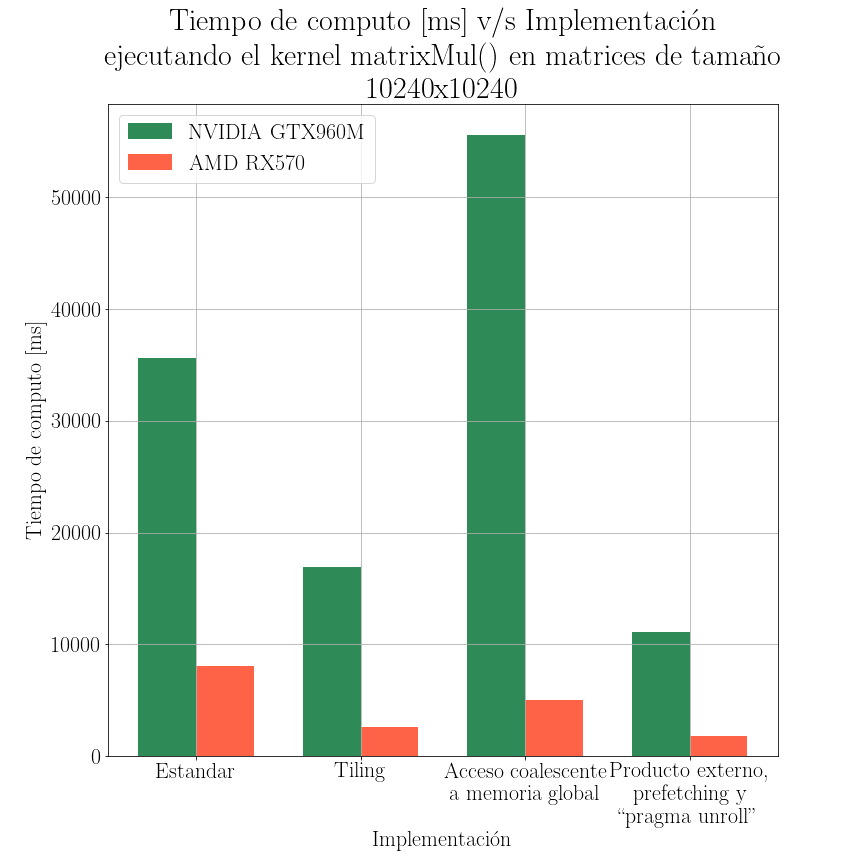
\includegraphics[width=\linewidth]{Figures/plot2.png}
    \caption{} 
  \end{subfigure}%
  \begin{subfigure}{0.5\textwidth}
    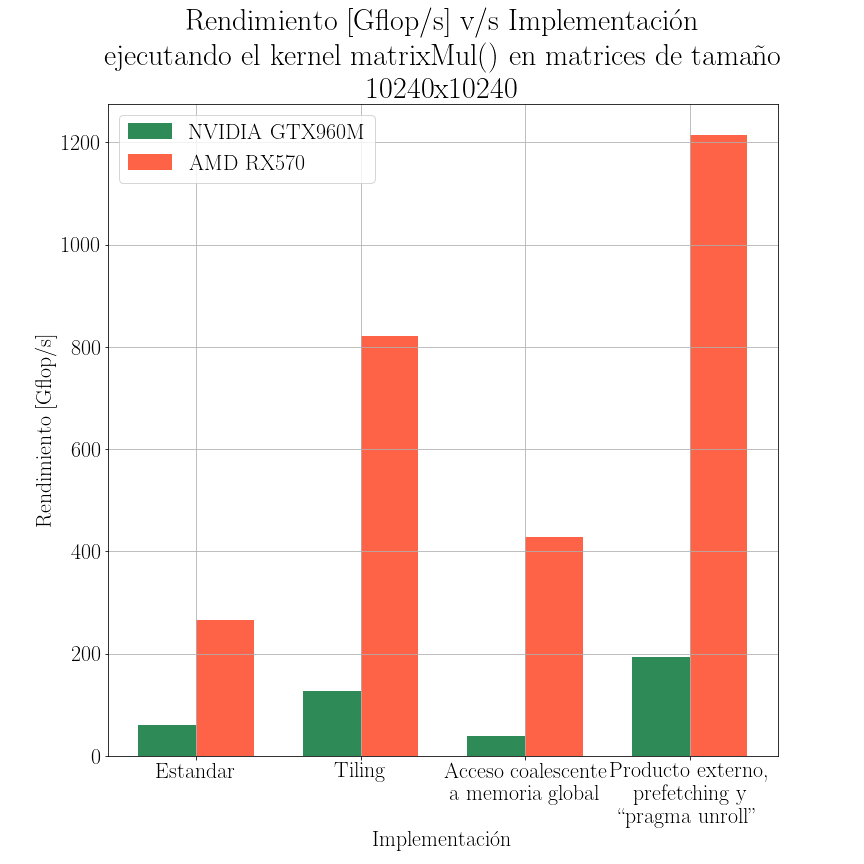
\includegraphics[width=\linewidth]{Figures/plot3.png}
    \caption{} 
  \end{subfigure}%
  \caption{Gráfico de tiempo de computo y rendimiento versus tamaño de vector al ejecutar el kernel matrixMul().}
  \label{fig:17}
\end{figure}

%------------------------

\newpage

Los resultados de la experimentación realizada sobre la implementación optimizada del método de Lattice Boltzmann se presentan en la Figura~\ref{fig:18}.
En dicha gráfica, se presentan los tiempos de ejecución por 20000 \textit{time steps} de 3 segundos reales cada uno, del código optimizado con 5 instancias (archivos) de entrada:

\begin{itemize}
    \item Iquique, correspondiente a niveles de agua de un tsunami registrado el año 2014 en la misma localidad, como grilla de \(549\times821\) nodos.
    \item Maule, correspondiente a niveles de agua de un tsunami registrado el año 2010 en la misma localidad, como grilla de \(158\times241\) nodos.
    \item Talinay, correspondiente a un datos de un tsunami ocurrido en la misma localidad, como grilla de \(124\times241\) nodos.
    \item Test40000, instancia de ejemplo del repositorio de LBM optimizado, de tamaño \(200\times200\) nodos.
    \item Test4000000, una instancia generada a partir de una función 
    \begin{equation*}
        f(x,y) = 5\exp\,\left(-50(0.013y^2 + 0.08125(x+0.5)^2)\right) + 1199
    \end{equation*}
    con $x,y \in [-2,2]\times[-2,2]$ en la que el dominio posee una ``costa'' para cada $x > 0.5$ de tamaño \(2000\times2000\) nodos.
\end{itemize}

En general, los resultados de ambas tarjetas gráficas siguen un mismo patrón en comparación a la magnitud del volumen de información entregado por los archivos de entrada para un mismo número de pasos del método de Lattice Boltzmann.
Los archivos de salida de las versiones del código para AMD y NVIDIA producen los mismos archivos, cuyos gráficos de calor se presentan en las 
% Figuras~\ref{fig:20},\ref{fig:21},\ref{fig:22},\ref{fig:23},\ref{fig:24}.
Figuras~\ref{fig:20}-\ref{fig:24}.
El rango del mapa de calor de las imágenes se define en base a la media de los niveles de agua presenten en todos los archivos de salida a graficar.

\begin{figure}[H]
  \centering
    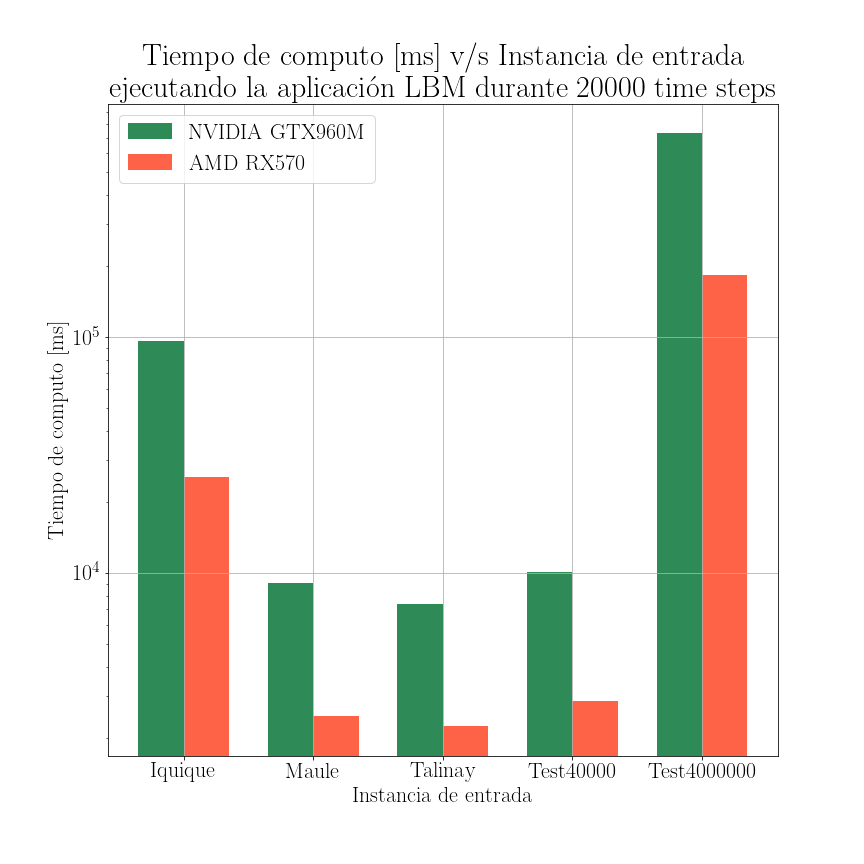
\includegraphics[width=0.8\linewidth]{Figures/plot4.png}
  \caption{Gráfico de tiempo de computo versus archivo de entrada al ejecutar el código optimizado de LBM por 20000 \textit{time steps}.}
  \label{fig:18}
\end{figure}

Los resultados de tiempos de computo por cada ``sub kernel'' generado sobre el kernel original del código \textit{LBM Framework} se presentan en los gráfico de la Figura~\ref{fig:19-1} y \ref{fig:19-2}, para CUDA y ROCm.
Se ejecutaron 10000 \textit{time steps} de archivos de entrada, representando instancias de nodos cuadrada, en donde un aumento en el tamaño del lado de forma exponencial es la única diferencia entre los archivos.
La situación simulada, esta compuesta por una superficie de agua modelada por la función
\begin{equation*}
    0.1\exp\left(-50(x^2 + y^2)\right) + 50
\end{equation*}
con $x,y \in [-4,4]\times[-4,4]$
Además, no se aplicaron condiciones de borde extra además de aquellas presentes en los bordes de la grilla.

A partir de lo que se observa, se puede notar que tan solo existen diferencias significativas en el primer y tercer kernels a lo largo de todos las ejecuciones de ambos diseños de arreglos \(f_1\) y \(f_2\).
Esto se debe a que en el segundo kernel no hay accesos al arreglo \(f_1\) o \(f_2\).
Esto implica que, en la ejecución de un framework generalizado no afecta de manera significativa el acceso coalescente a la memoria, por lo menos al hacer uso de GPU's de venta en mercado general (computadoras personales).
Sin embargo, se debe recalcar que al momento de ejecutar un software de este tipo con inputs de volumen mucho mayor, la diferencia de tiempo presente se hace cada vez notable, por lo que esta si debiera ser significativa al utilizar clústers de nodos de procesamiento o supercomputadoras con GPU's de características de gran magnitud.


\begin{figure}[H]
  \centering
  \begin{subfigure}{0.5\textwidth}
    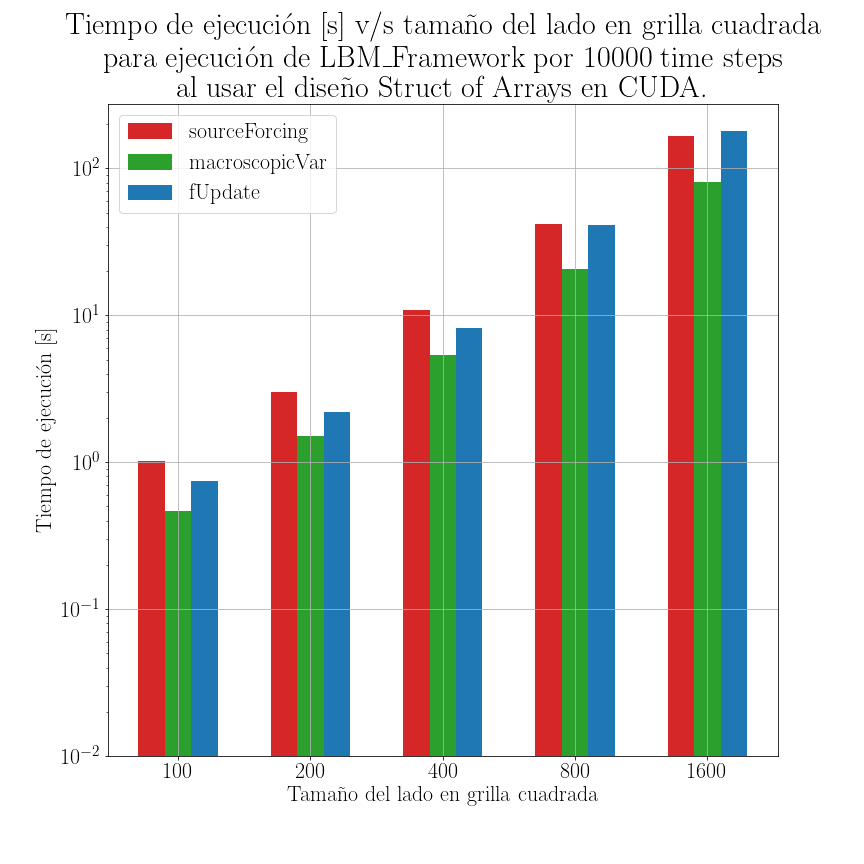
\includegraphics[width=\linewidth]{Figures/plot6.png}
    \caption{} 
  \end{subfigure}%
  \begin{subfigure}{0.5\textwidth}
    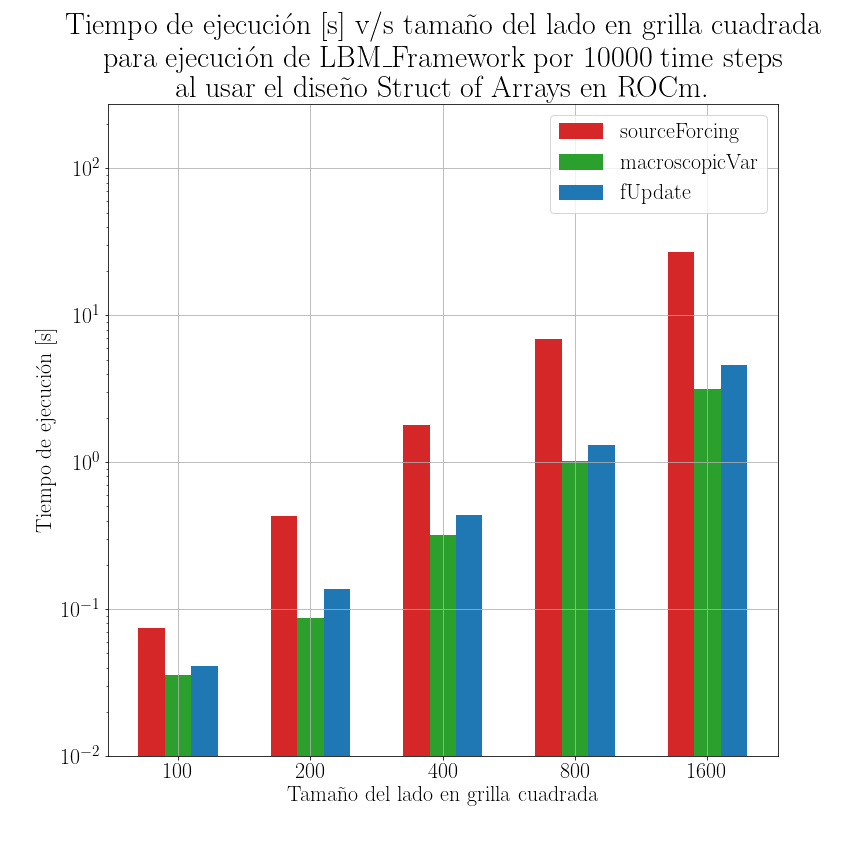
\includegraphics[width=\linewidth]{Figures/plot8.png}
    \caption{} 
  \end{subfigure}%
  \caption{Gráfico de tiempo de cómputo versus tamaño de archivo input ejecutando el código \textit{LBM Framework} por 10000 \textit{time steps} usando SoA y AoS en el diseño de los arreglos \(f_1\) y \(f_2\) en CUDA.}
  \label{fig:19-1}
\end{figure}

\begin{figure}[H]
  \centering
  \begin{subfigure}{0.5\textwidth}
    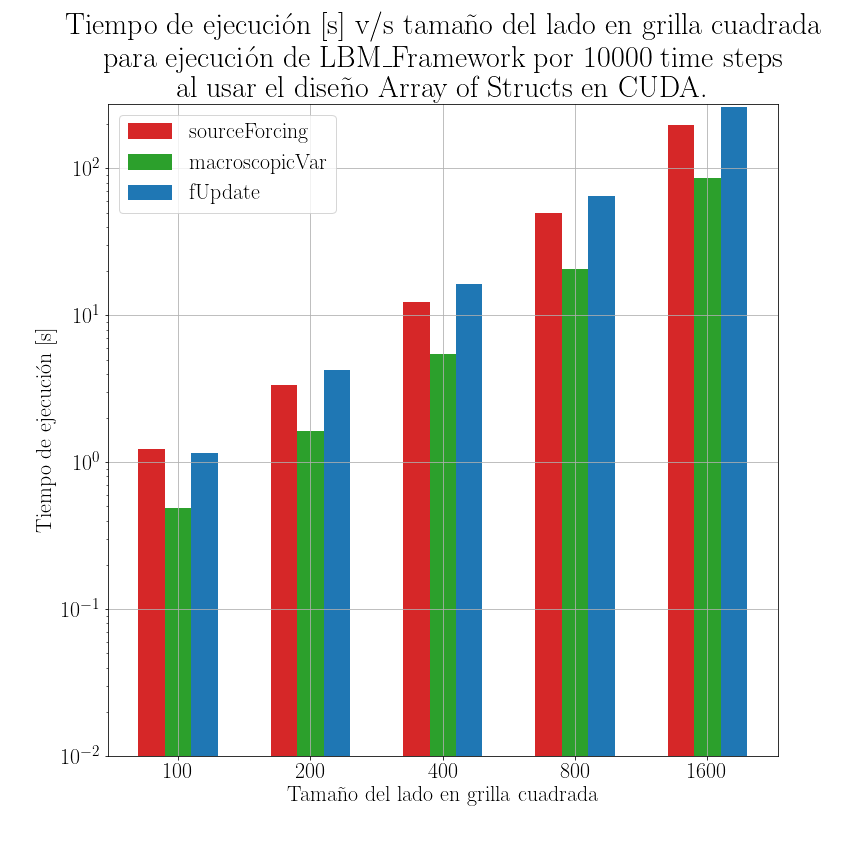
\includegraphics[width=\linewidth]{Figures/plot7.png}
    \caption{} 
  \end{subfigure}%
  \begin{subfigure}{0.5\textwidth}
    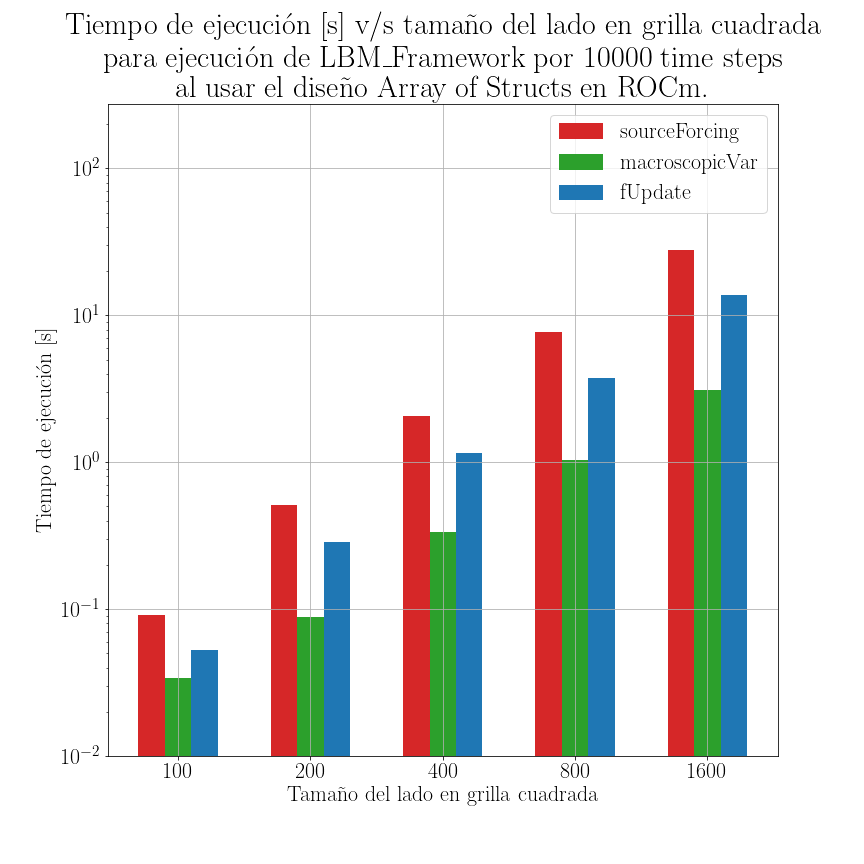
\includegraphics[width=\linewidth]{Figures/plot9.png}
    \caption{} 
  \end{subfigure}%
  \caption{Gráfico de tiempo de cómputo versus tamaño de archivo input ejecutando el código \textit{LBM Framework} por 10000 \textit{time steps} usando SoA y AoS en el diseño de los arreglos \(f_1\) y \(f_2\) en ROCm.}
  \label{fig:19-2}
\end{figure}

%

Con tal de cumplir el objetivo que buscaba proponer instancias de posibles tsunamis en costas Chilenas, es que se presentan las 
Figuras~\ref{fig:25}-\ref{fig:27}.
Estas situaciones corresponden a niveles de agua generados a partir de funciones similares a las de instancias anteriores, correspondientes a:

\begin{itemize}
    \item \textbf{Antofagasta}, que simulan las costas de la ciudad de Antofagasta desde las latitudes 23°23'36.6"S a 24°03'40.7"S aproximadamente. 
    Los niveles de agua están modelados por la función
    \begin{equation*}
        f(x,y) = 5\,\exp\left(-50(0.08x^2 + 0.25(y+1)^2)\right) + 500
    \end{equation*}
    con \(x,y\in[-3,3]\times[-3,-3]\) y una rotación antihoraria de 30°.
    \item \textbf{Serena}, que simulan las costas de la ciudad de La Serena desde las latitudes 29°29'31.8"S a 30°27'32.6"S aproximadamente.
    Los niveles de agua están modelados por la función
    \begin{equation*}
        f(x,y) = 5\,\exp\left(-50(0.25x^2 + 0.25(y+1)^2)\right) + 500
    \end{equation*}
    con \(x,y\in[-3,3]\times[-3,-3]\).
    \item \textbf{Valparaiso}, que simulan el litoral central Chileno desde las latitudes 31°54'00.3"S a 34°20'33.8"S aproximadamente.
    Los niveles de agua están modelados por la función
    \begin{equation*}
        f(x,y) = 5\,\exp\left(-50(0.08x^2 + 0.005(y+1)^2)\right) + 500
    \end{equation*}
    con \(x,y\in[0,6]\times[-3,-3]\).
\end{itemize}

En estas simulaciones realizadas, cada \textit{time step} corresponde a 3 segundos reales.

%--------------------------------------------



\begin{figure}[H]
\centering
\begin{subfigure}[b]{.4\linewidth}
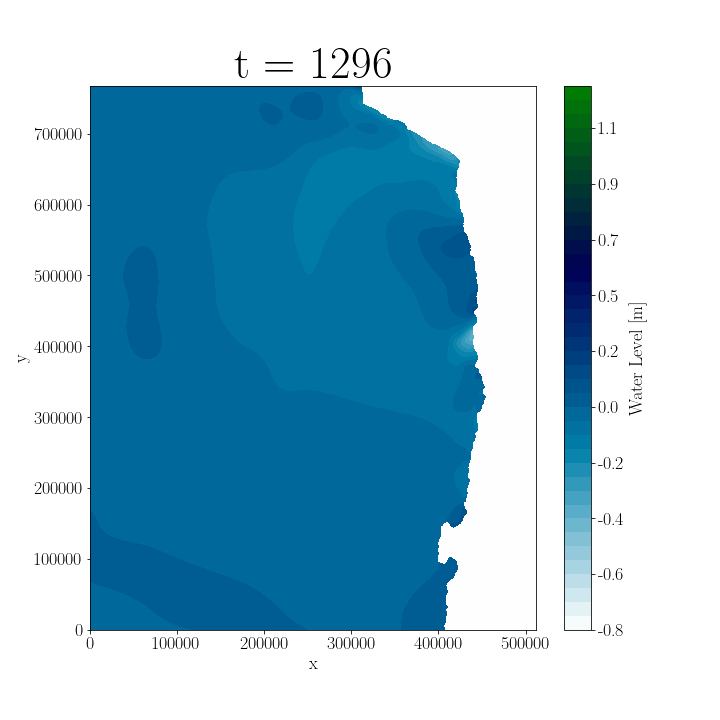
\includegraphics[width=\linewidth]{Figures/1-1.png}
\caption{}
\end{subfigure}
\begin{subfigure}[b]{.4\linewidth}
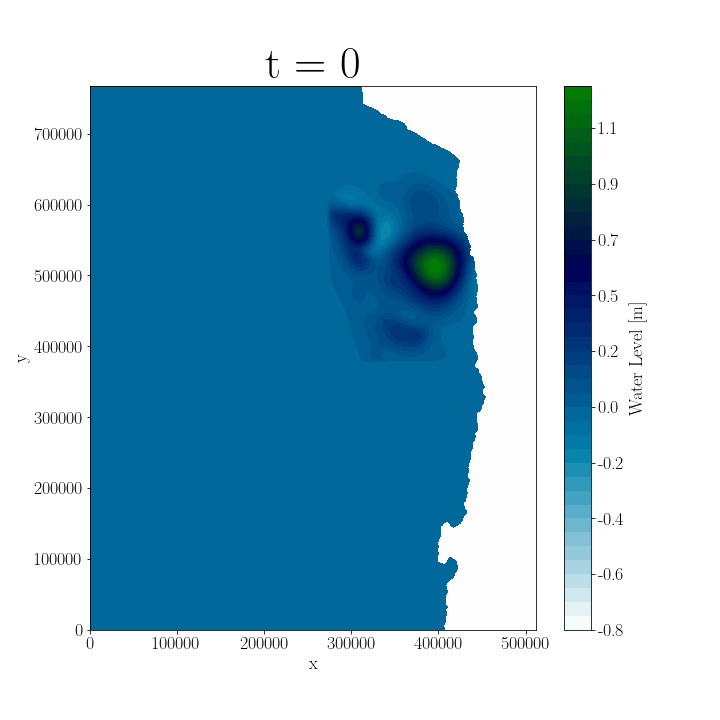
\includegraphics[width=\linewidth]{Figures/1-2.png}
\caption{}
\end{subfigure}

\begin{subfigure}[b]{.4\linewidth}
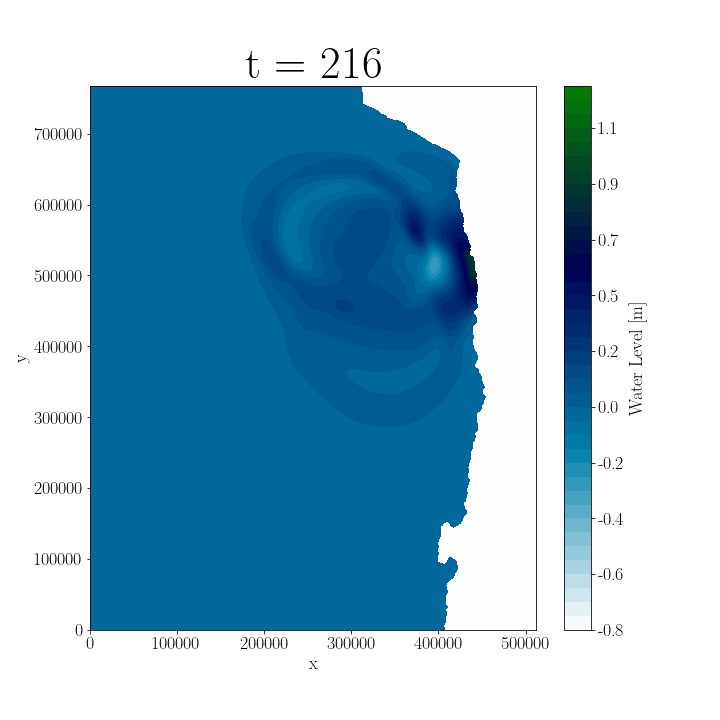
\includegraphics[width=\linewidth]{Figures/1-3.png}
\caption{}
\end{subfigure}
\begin{subfigure}[b]{.4\linewidth}
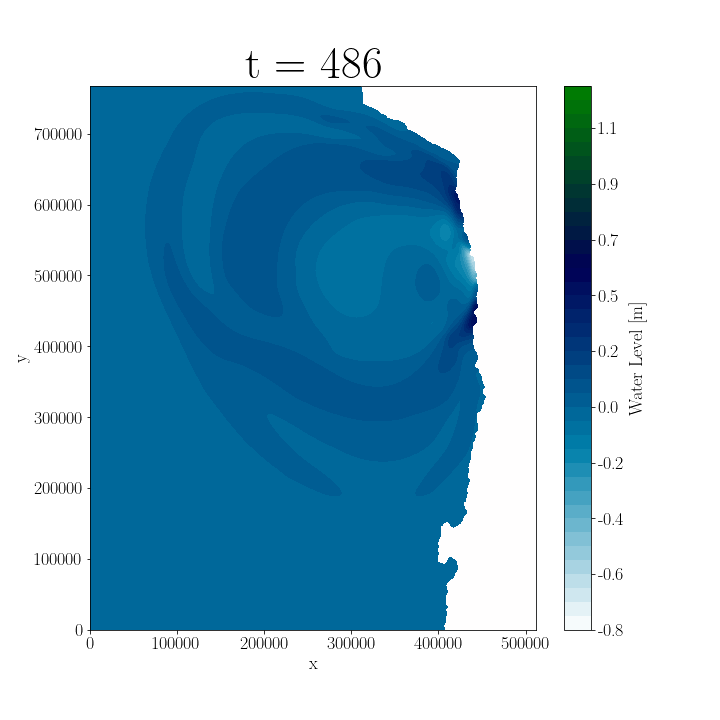
\includegraphics[width=\linewidth]{Figures/1-4.png}
\caption{}
\end{subfigure}

\begin{subfigure}[b]{.4\linewidth}
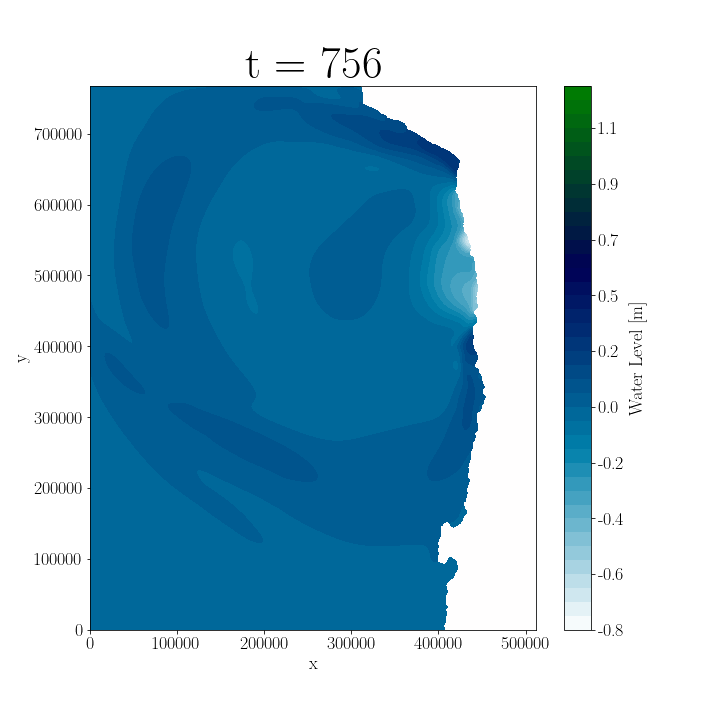
\includegraphics[width=\linewidth]{Figures/1-5.png}
\caption{}
\end{subfigure}
\begin{subfigure}[b]{.4\linewidth}
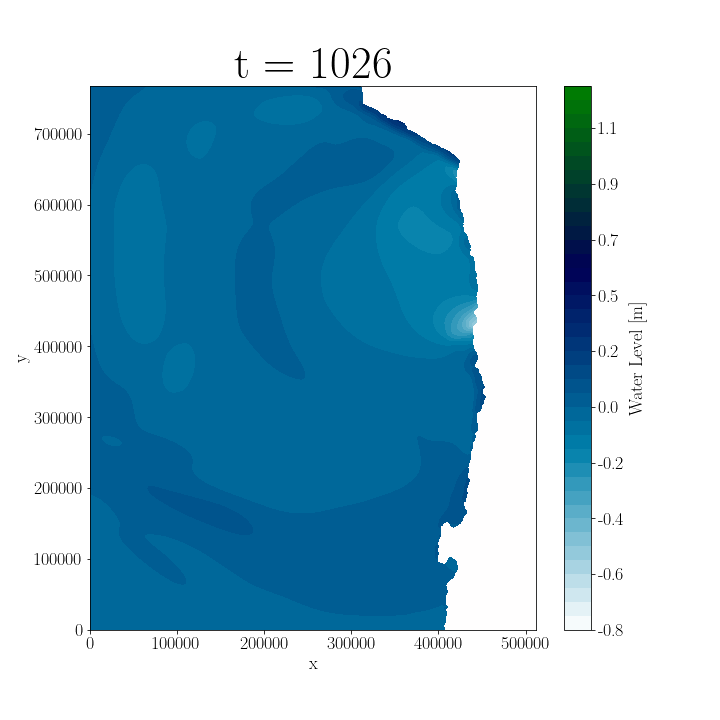
\includegraphics[width=\linewidth]{Figures/1-6.png}
\caption{}
\end{subfigure}


\caption{Niveles de agua de la salida de ejecutar el código de LBM optimizado con el archivo de entrada \textbf{Iquique}.}
\label{fig:20}
\end{figure}

%--------------------------------------------

\begin{figure}[H]
\centering
\begin{subfigure}[b]{.4\linewidth}
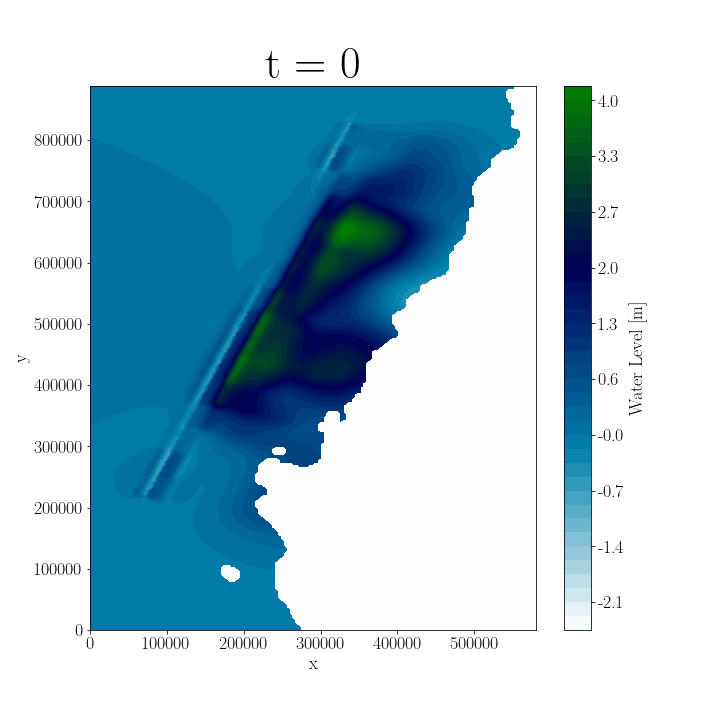
\includegraphics[width=\linewidth]{Figures/2-1.png}
\caption{}
\end{subfigure}
\begin{subfigure}[b]{.4\linewidth}
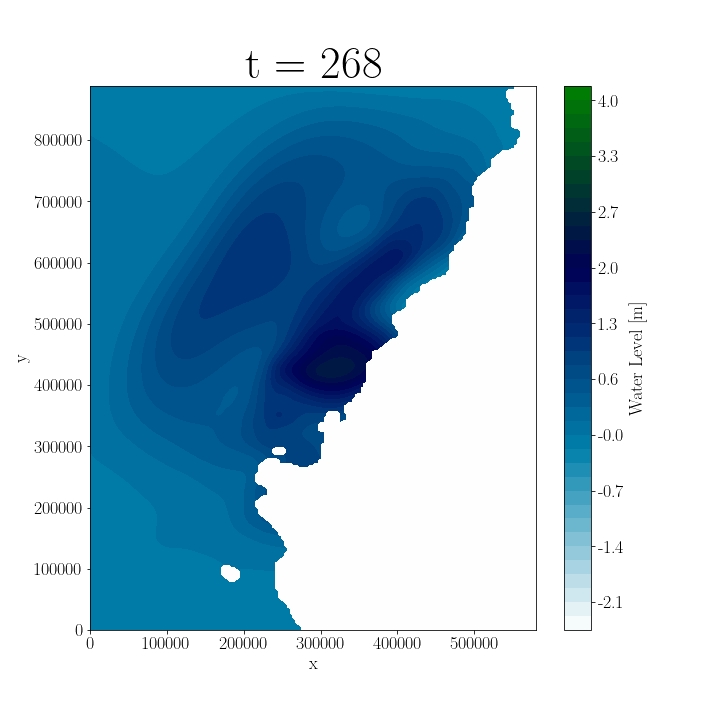
\includegraphics[width=\linewidth]{Figures/2-2.png}
\caption{}
\end{subfigure}

\begin{subfigure}[b]{.4\linewidth}
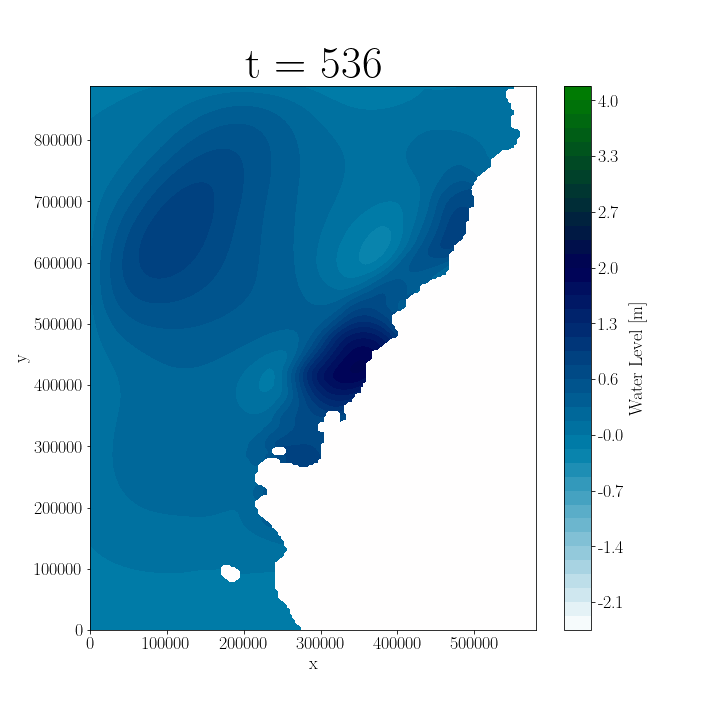
\includegraphics[width=\linewidth]{Figures/2-3.png}
\caption{}
\end{subfigure}
\begin{subfigure}[b]{.4\linewidth}
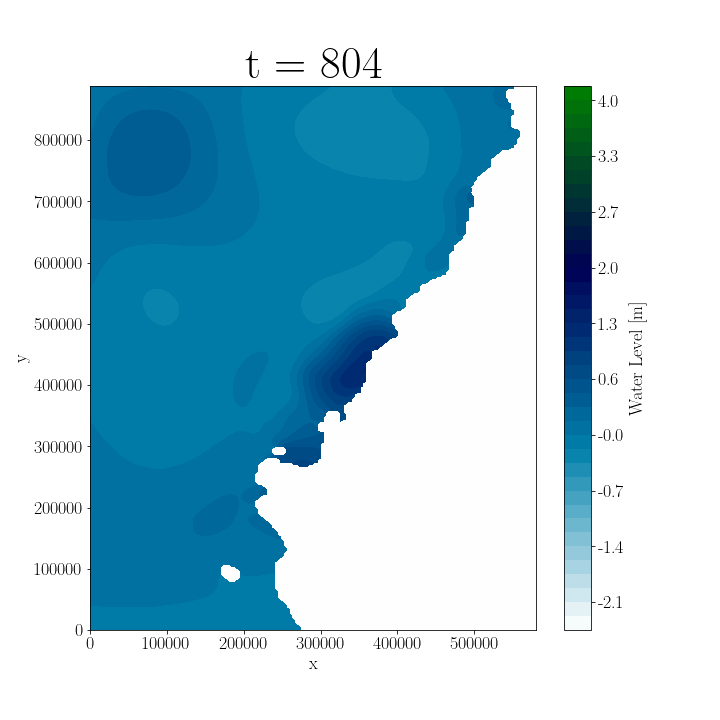
\includegraphics[width=\linewidth]{Figures/2-4.png}
\caption{}
\end{subfigure}

\begin{subfigure}[b]{.4\linewidth}
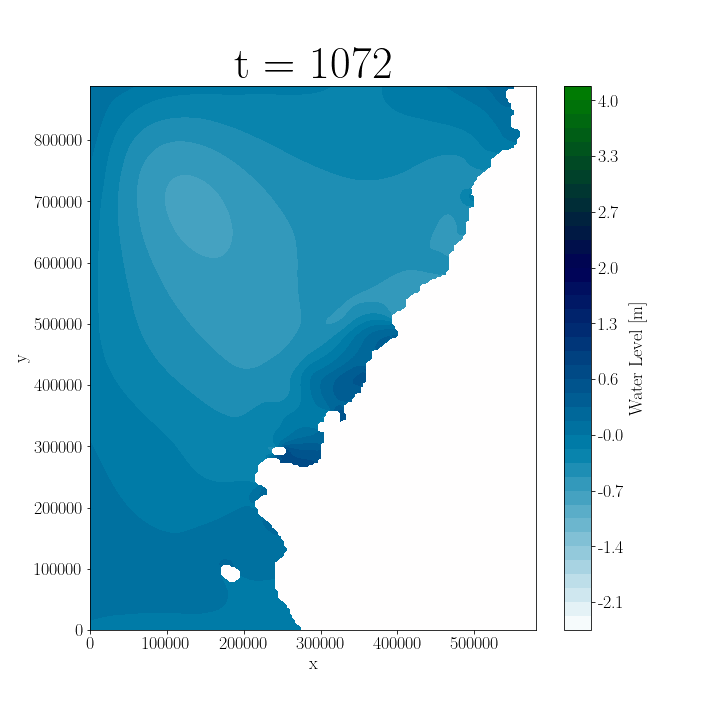
\includegraphics[width=\linewidth]{Figures/2-5.png}
\caption{}
\end{subfigure}
\begin{subfigure}[b]{.4\linewidth}
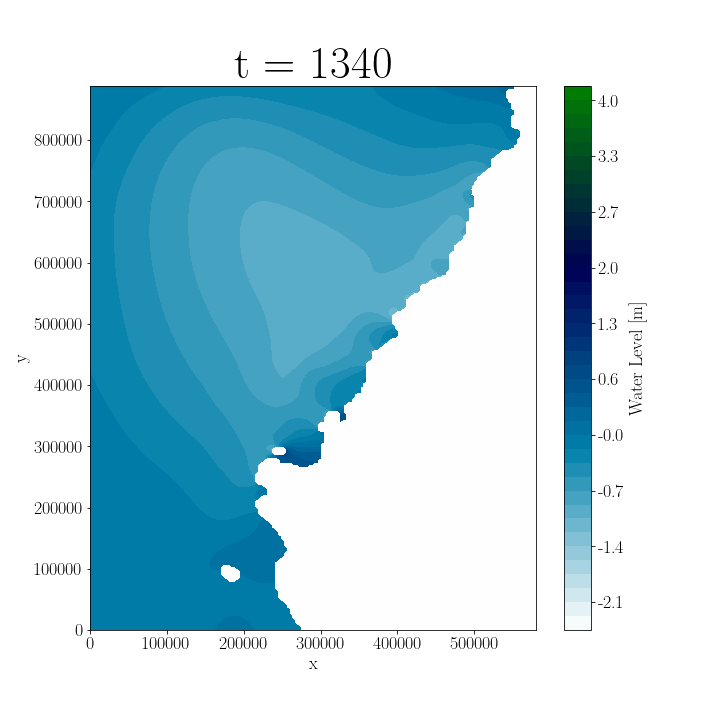
\includegraphics[width=\linewidth]{Figures/2-6.png}
\caption{}
\end{subfigure}
\caption{Niveles de agua de la salida de ejecutar el código de LBM optimizado con el archivo de entrada \textbf{Maule}.}
\label{fig:21}
\end{figure}

%--------------------------------------------

\begin{figure}[H]
\centering
\begin{subfigure}[b]{.4\linewidth}
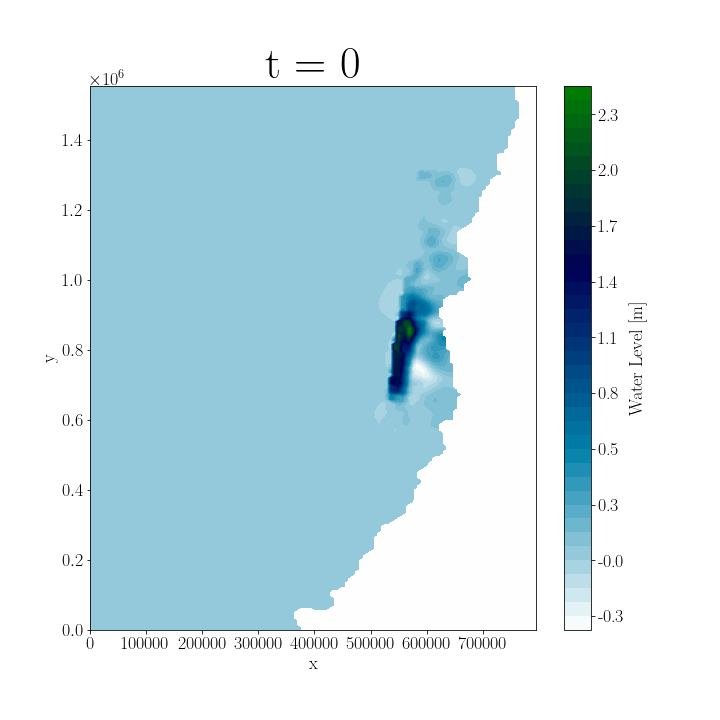
\includegraphics[width=\linewidth]{Figures/3-1.png}
\caption{}
\end{subfigure}
\begin{subfigure}[b]{.4\linewidth}
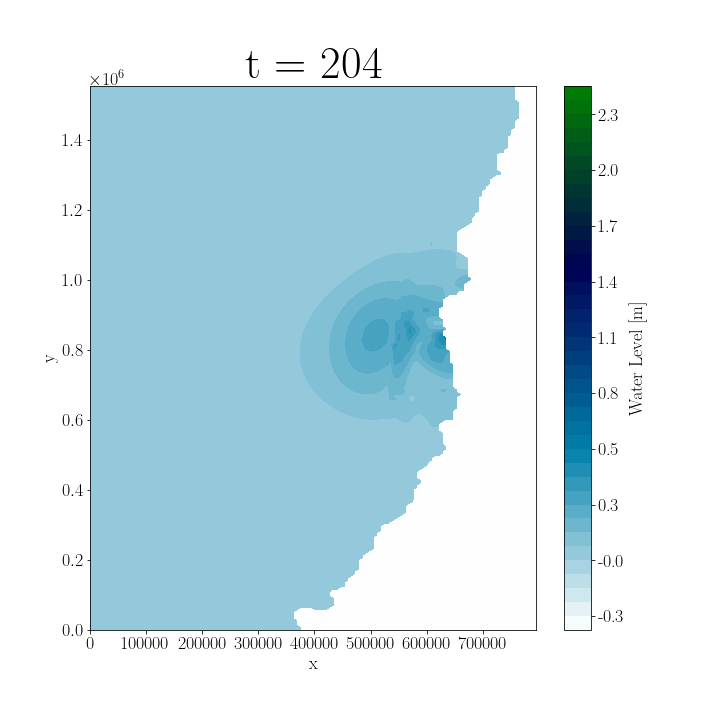
\includegraphics[width=\linewidth]{Figures/3-2.png}
\caption{}
\end{subfigure}

\begin{subfigure}[b]{.4\linewidth}
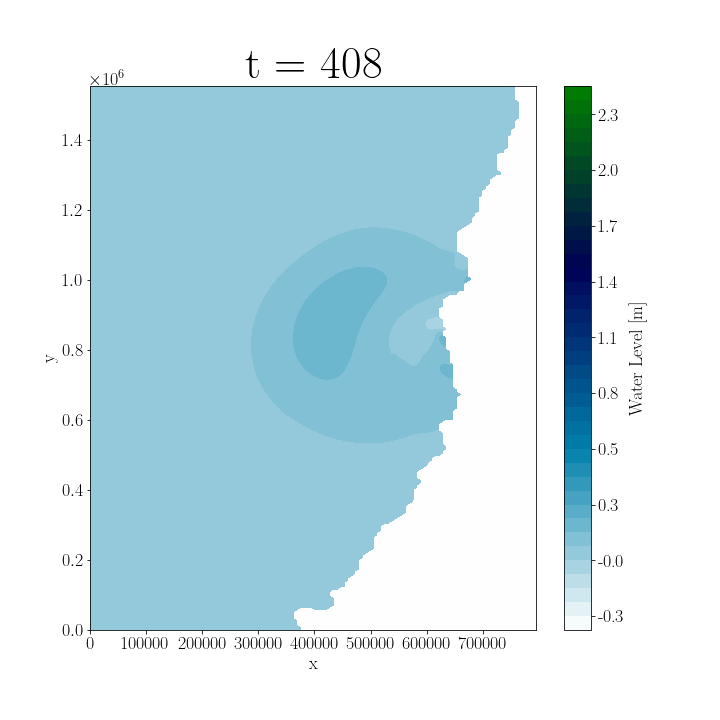
\includegraphics[width=\linewidth]{Figures/3-3.png}
\caption{}
\end{subfigure}
\begin{subfigure}[b]{.4\linewidth}
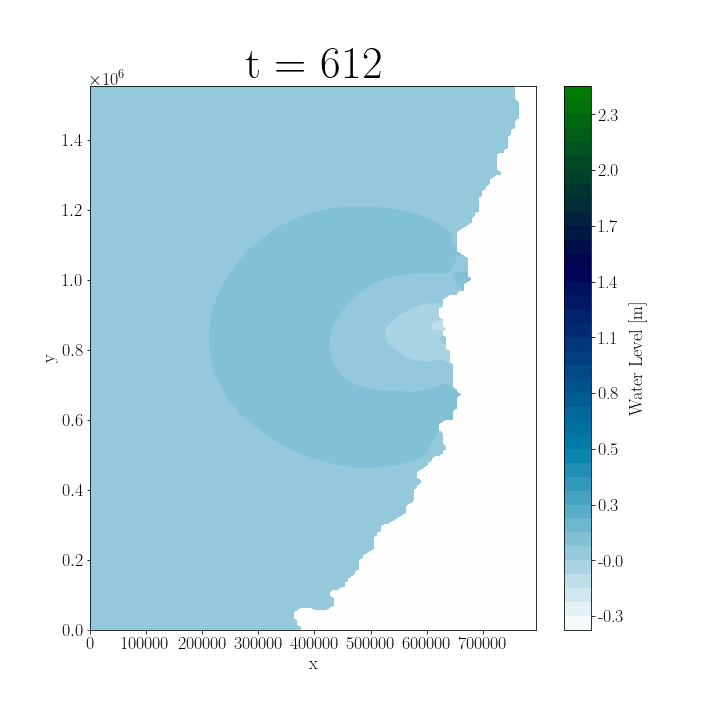
\includegraphics[width=\linewidth]{Figures/3-4.png}
\caption{}
\end{subfigure}

\begin{subfigure}[b]{.4\linewidth}
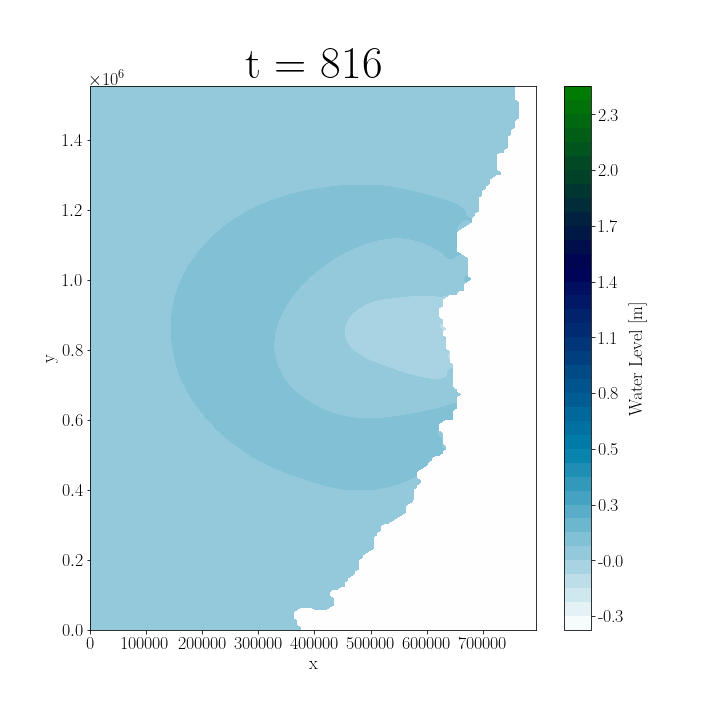
\includegraphics[width=\linewidth]{Figures/3-5.png}
\caption{}
\end{subfigure}
\begin{subfigure}[b]{.4\linewidth}
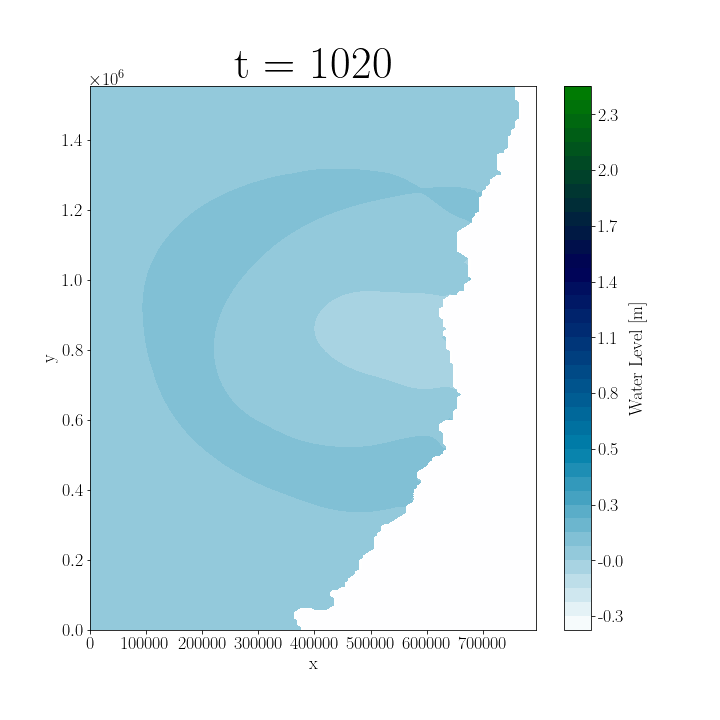
\includegraphics[width=\linewidth]{Figures/3-6.png}
\caption{}
\end{subfigure}
\caption{Niveles de agua de la salida de ejecutar el código de LBM optimizado con el archivo de entrada \textbf{Talinay}.}
\label{fig:22}
\end{figure}

%--------------------------------------------

\begin{figure}[H]
\centering
\begin{subfigure}[b]{.4\linewidth}
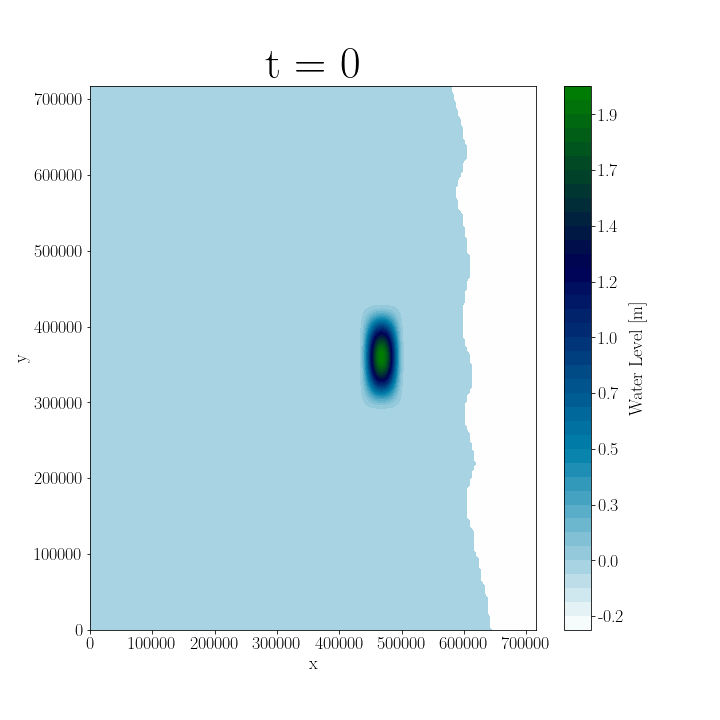
\includegraphics[width=\linewidth]{Figures/4-1.png}
\caption{}
\end{subfigure}
\begin{subfigure}[b]{.4\linewidth}
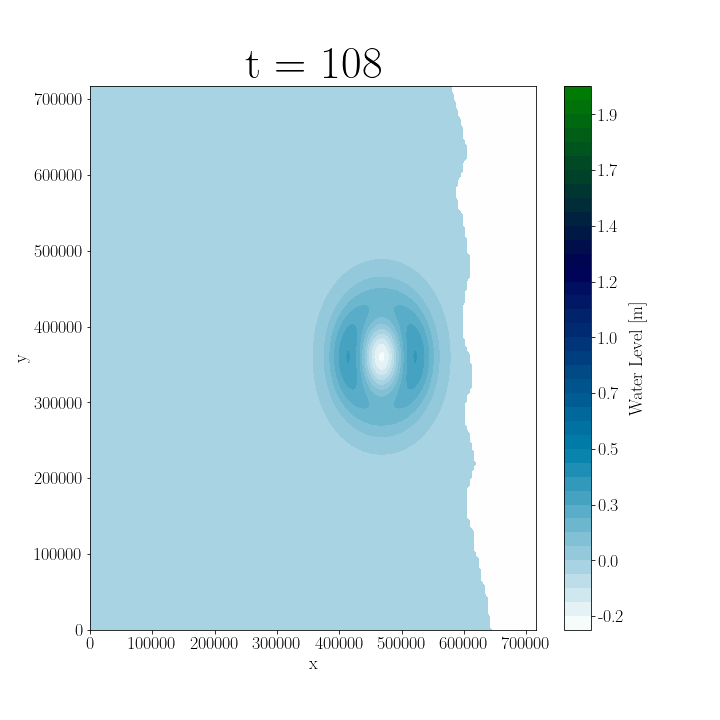
\includegraphics[width=\linewidth]{Figures/4-2.png}
\caption{}
\end{subfigure}

\begin{subfigure}[b]{.4\linewidth}
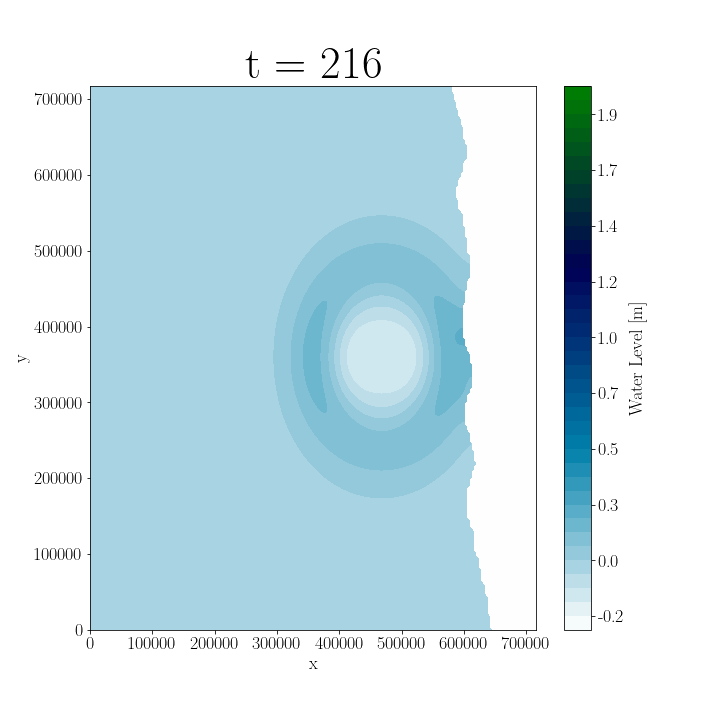
\includegraphics[width=\linewidth]{Figures/4-3.png}
\caption{}
\end{subfigure}
\begin{subfigure}[b]{.4\linewidth}
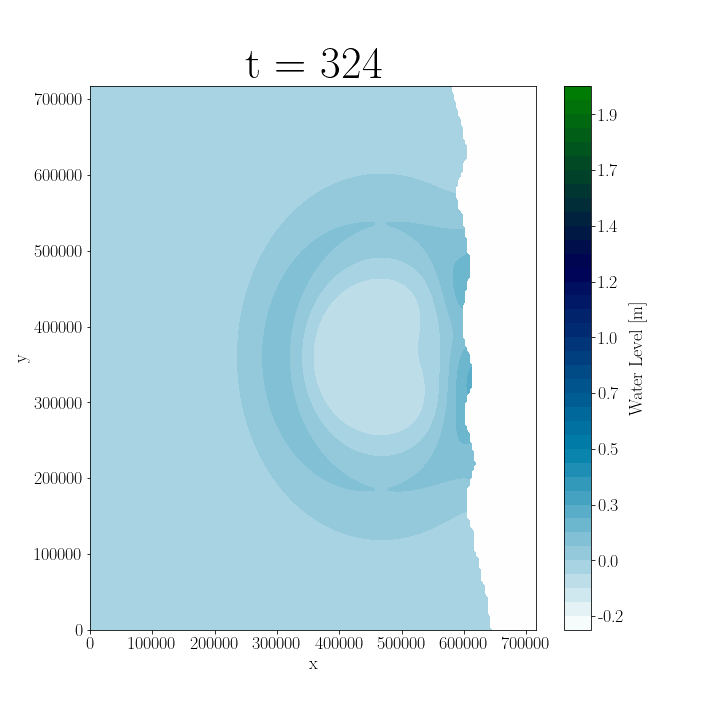
\includegraphics[width=\linewidth]{Figures/4-4.png}
\caption{}
\end{subfigure}

\begin{subfigure}[b]{.4\linewidth}
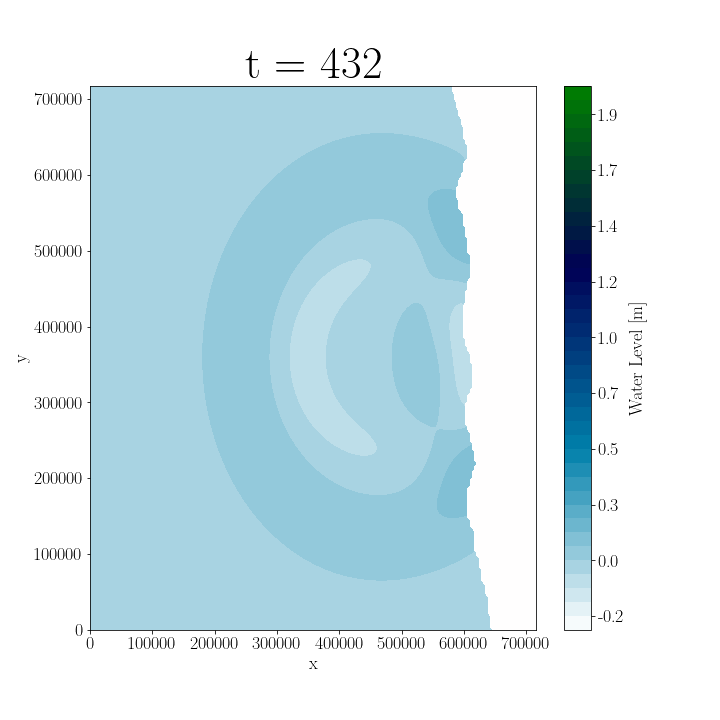
\includegraphics[width=\linewidth]{Figures/4-5.png}
\caption{}
\end{subfigure}
\begin{subfigure}[b]{.4\linewidth}
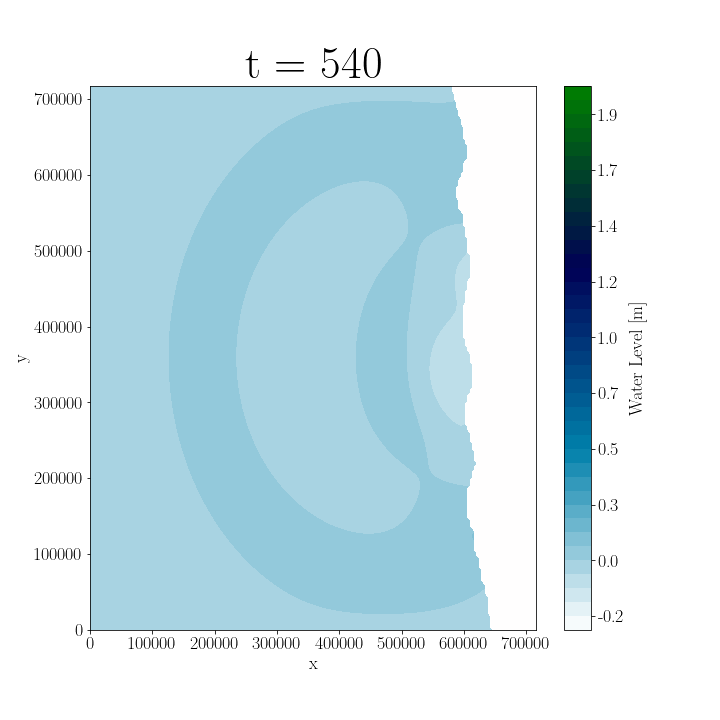
\includegraphics[width=\linewidth]{Figures/4-6.png}
\caption{}
\end{subfigure}

\caption{Niveles de agua de la salida de ejecutar el código de LBM optimizado con el archivo de entrada \textbf{Test40000}.}
\label{fig:23}
\end{figure}

%--------------------------------------------

\begin{figure}[H]
\centering
\begin{subfigure}[b]{.4\linewidth}
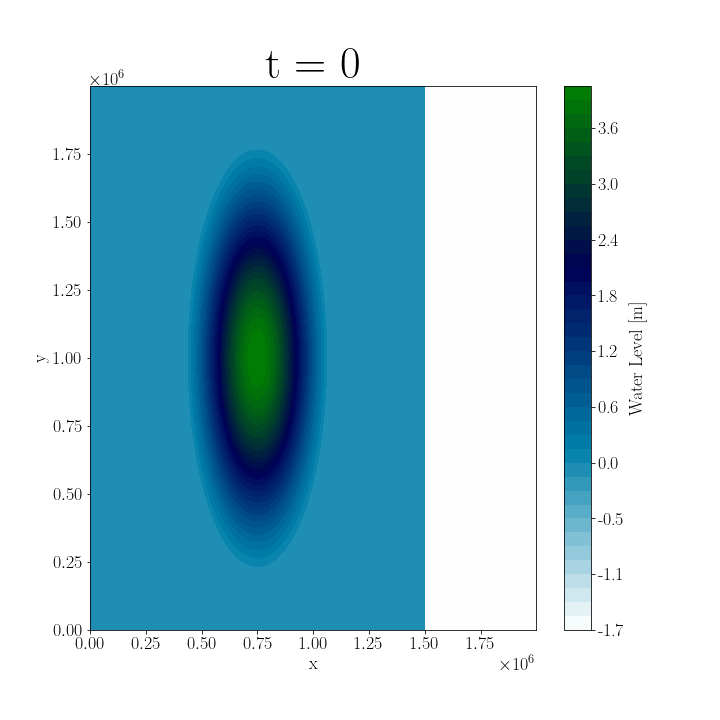
\includegraphics[width=\linewidth]{Figures/5-1.png}
\caption{}
\end{subfigure}
\begin{subfigure}[b]{.4\linewidth}
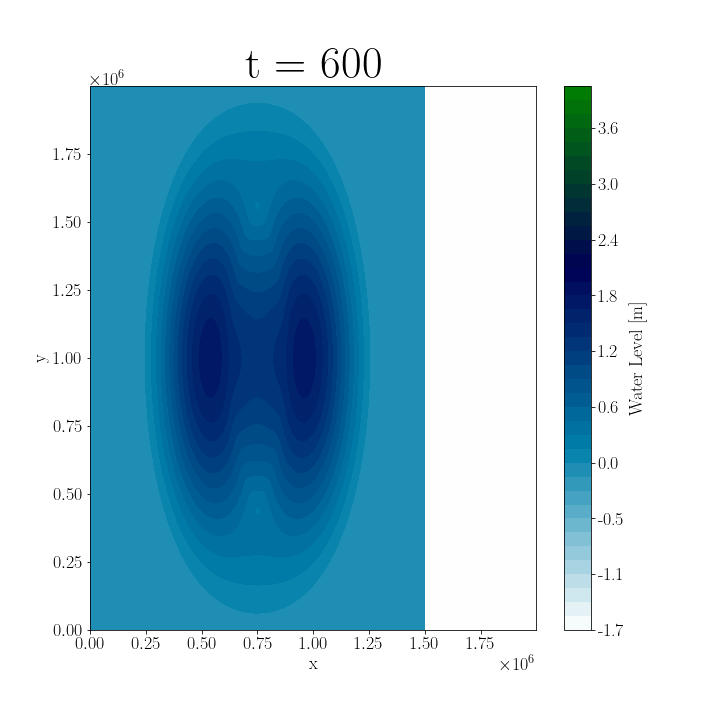
\includegraphics[width=\linewidth]{Figures/5-2.png}
\caption{}
\end{subfigure}

\begin{subfigure}[b]{.4\linewidth}
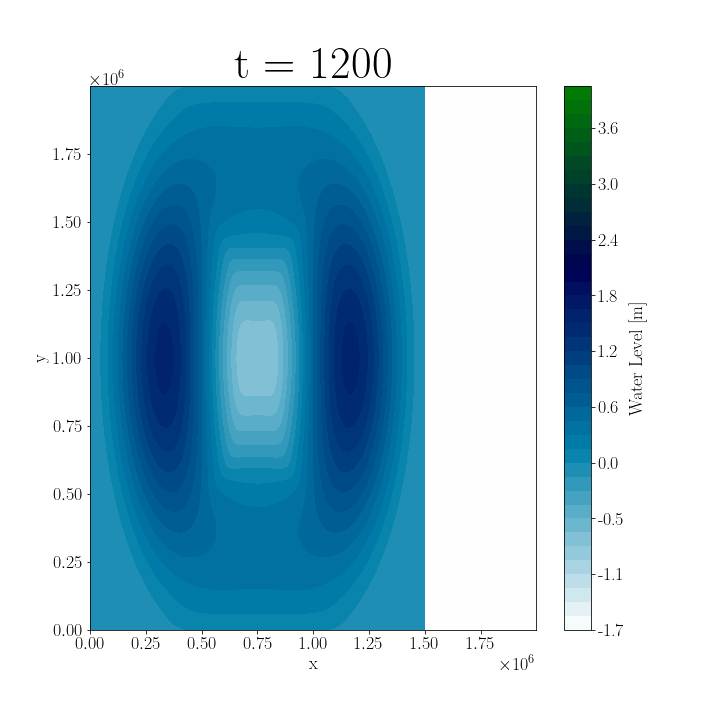
\includegraphics[width=\linewidth]{Figures/5-3.png}
\caption{}
\end{subfigure}
\begin{subfigure}[b]{.4\linewidth}
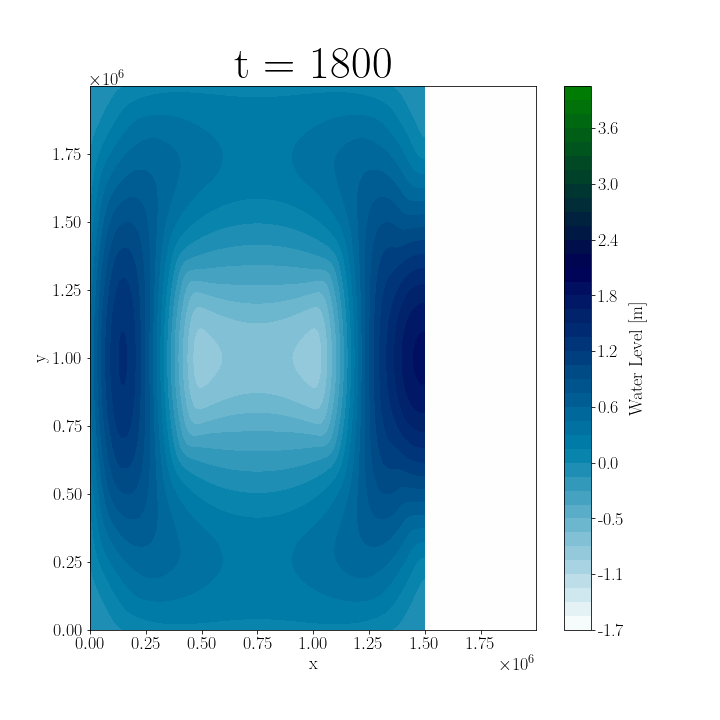
\includegraphics[width=\linewidth]{Figures/5-4.png}
\caption{}
\end{subfigure}

\begin{subfigure}[b]{.4\linewidth}
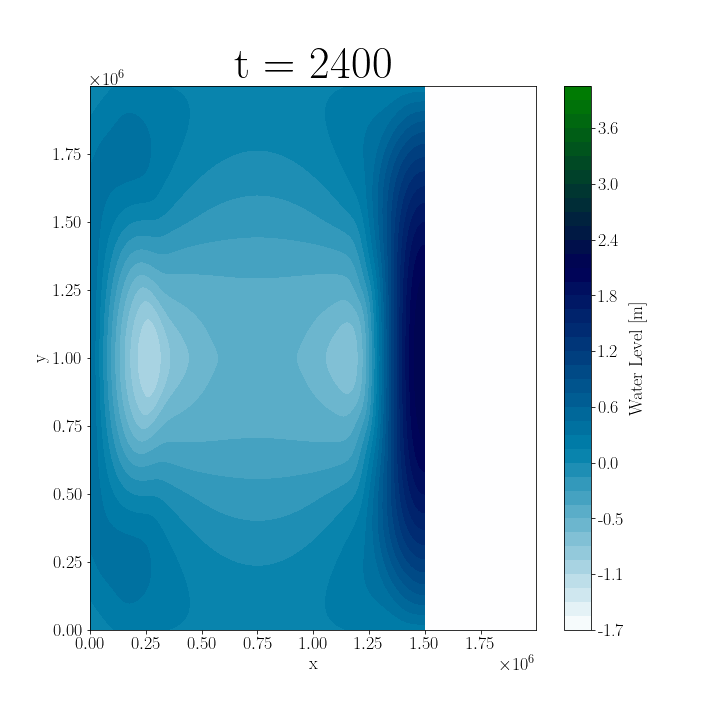
\includegraphics[width=\linewidth]{Figures/5-5.png}
\caption{}
\end{subfigure}
\begin{subfigure}[b]{.4\linewidth}
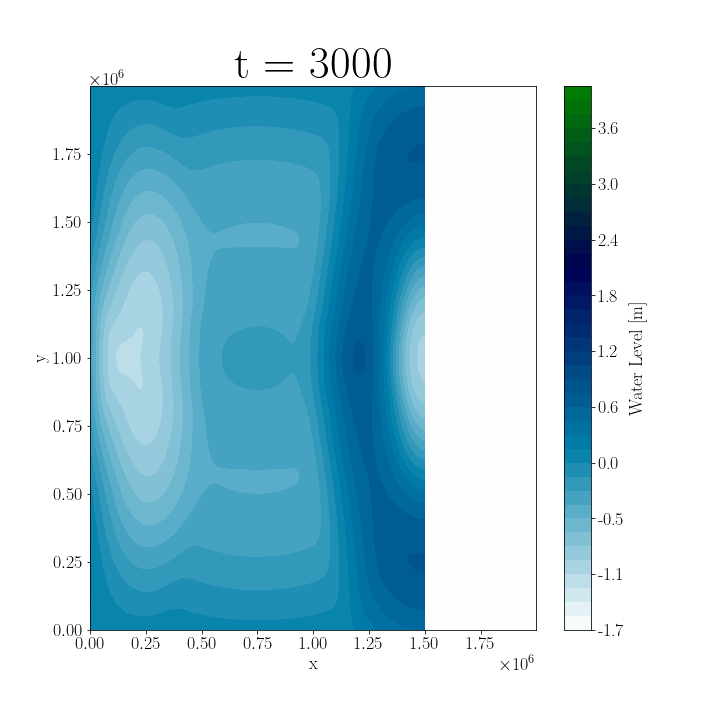
\includegraphics[width=\linewidth]{Figures/5-6.png}
\caption{}
\end{subfigure}
\caption{Niveles de agua de la salida de ejecutar el código de LBM optimizado con el archivo de entrada \textbf{Test40000}.}
\label{fig:24}
\end{figure}

%--------------------------------------------

\begin{figure}[H]
\centering
\begin{subfigure}[b]{.4\linewidth}
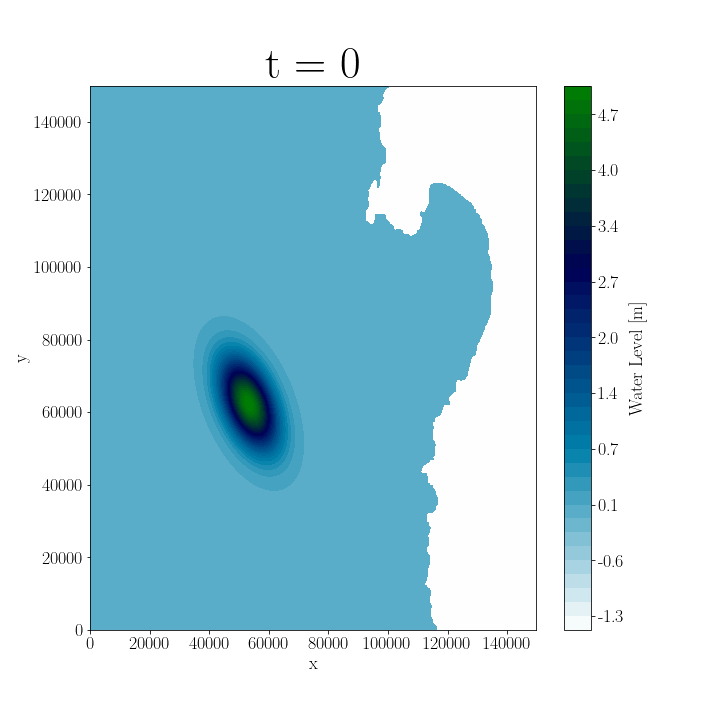
\includegraphics[width=\linewidth]{Figures/Plots/Antofa1.png}
\caption{desnivel máximo = 4.99 [m]}
\end{subfigure}
\begin{subfigure}[b]{.4\linewidth}
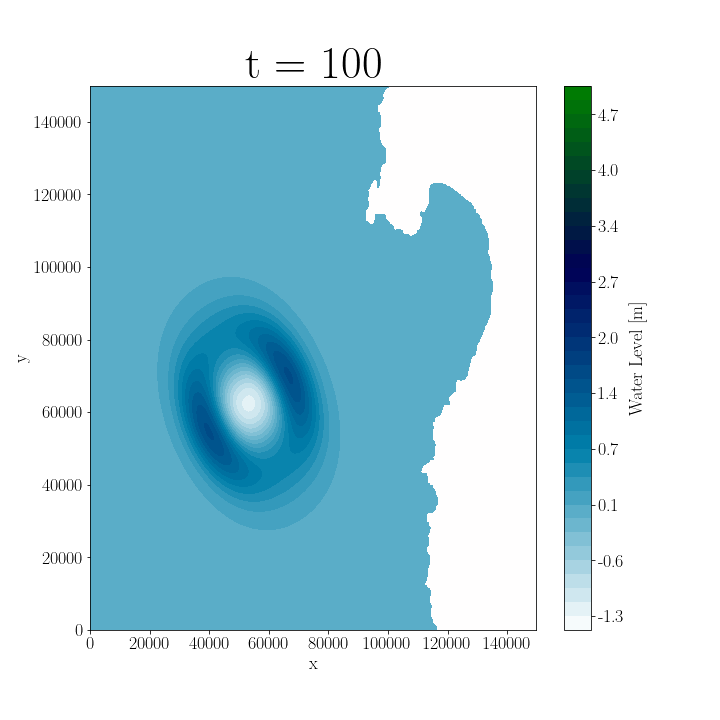
\includegraphics[width=\linewidth]{Figures/Plots/Antofa2.png}
\caption{desnivel máximo = 1.56 [m]}
\end{subfigure}

\begin{subfigure}[b]{.4\linewidth}
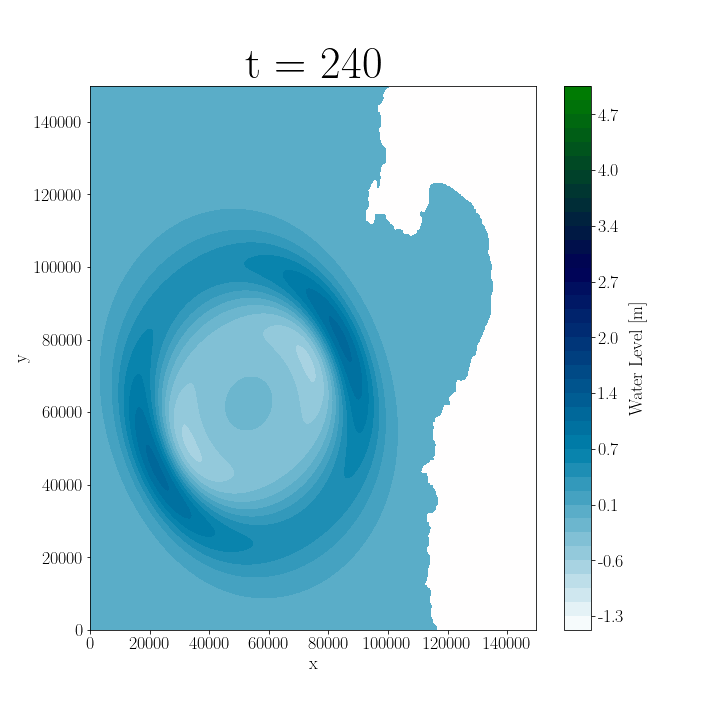
\includegraphics[width=\linewidth]{Figures/Plots/Antofa3.png}
\caption{desnivel máximo = 1.08 [m]}
\end{subfigure}
\begin{subfigure}[b]{.4\linewidth}
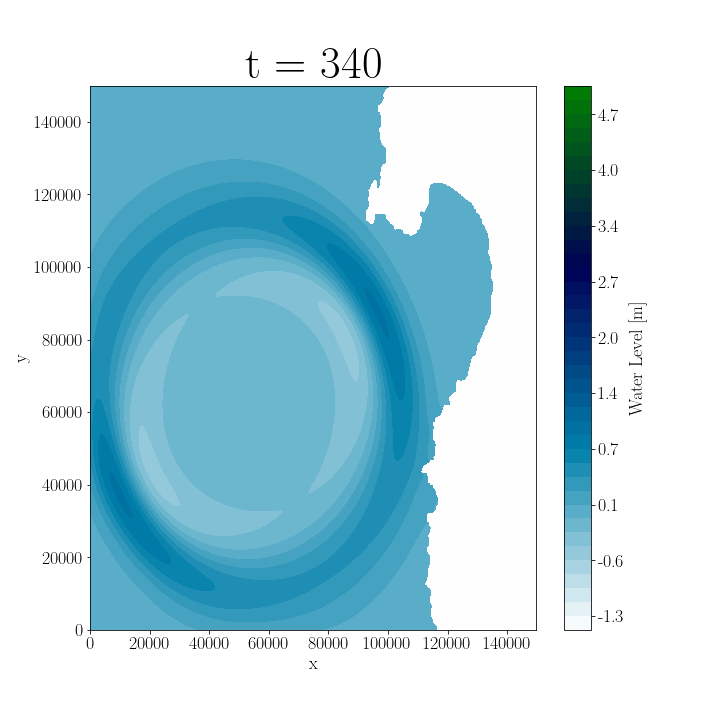
\includegraphics[width=\linewidth]{Figures/Plots/Antofa4.png}
\caption{desnivel máximo = 0.90 [m]}
\end{subfigure}

\begin{subfigure}[b]{.4\linewidth}
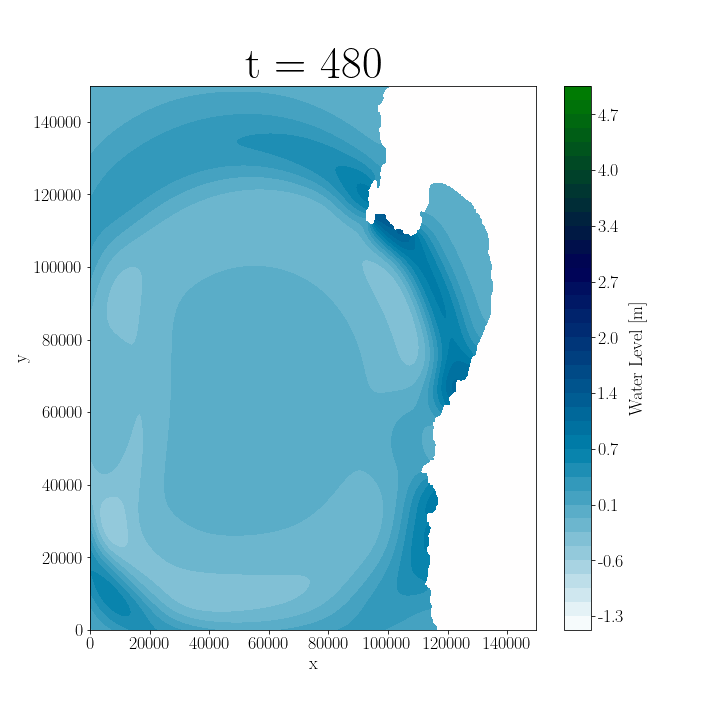
\includegraphics[width=\linewidth]{Figures/Plots/Antofa5.png}
\caption{desnivel máximo = 1.37 [m]}
\end{subfigure}
\begin{subfigure}[b]{.4\linewidth}
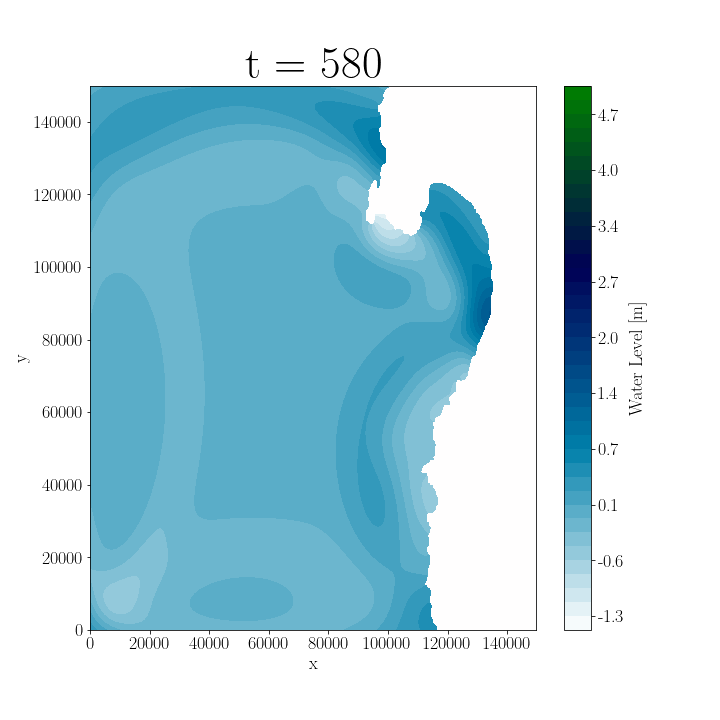
\includegraphics[width=\linewidth]{Figures/Plots/Antofa6.png}
\caption{desnivel máximo = 1.38 [m]}
\end{subfigure}
\caption{Niveles de agua de la salida de ejecutar el código de LBM optimizado con el archivo de entrada \textbf{Antofagasta}.}
\label{fig:25}
\end{figure}

%--------------------------------------------

\begin{figure}[H]
\centering
\begin{subfigure}[b]{.4\linewidth}
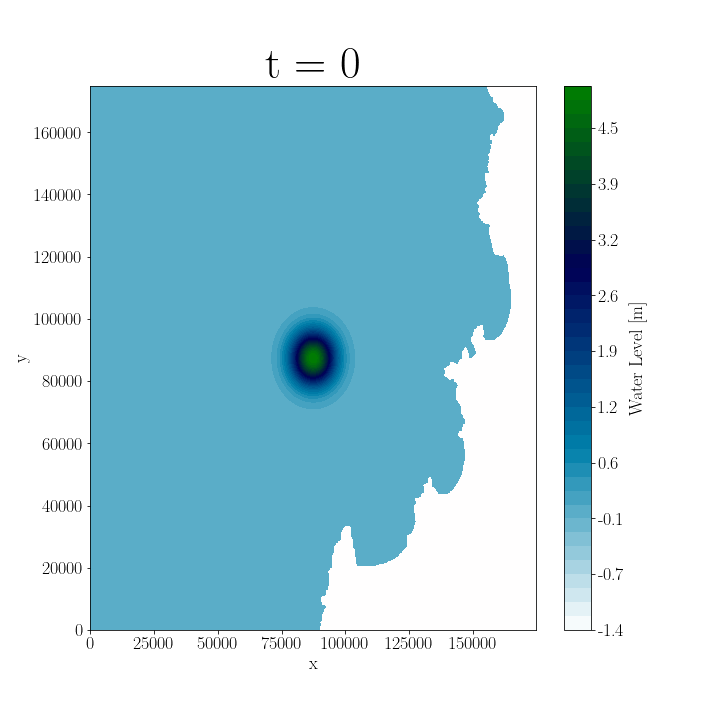
\includegraphics[width=\linewidth]{Figures/Plots/Serena1.png}
\caption{desnivel máximo = 4.99 [m]}
\end{subfigure}
\begin{subfigure}[b]{.4\linewidth}
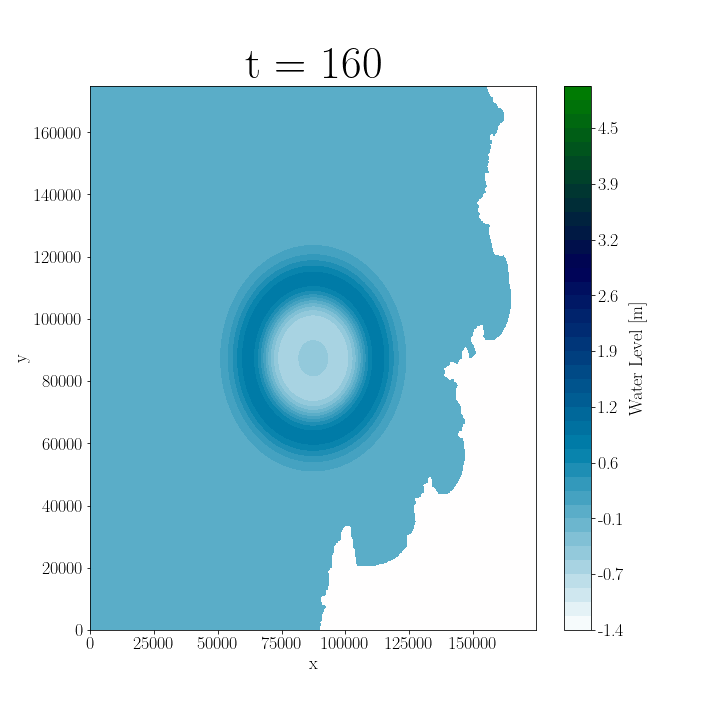
\includegraphics[width=\linewidth]{Figures/Plots/Serena2.png}
\caption{desnivel máximo = 0.83 [m]}
\end{subfigure}

\begin{subfigure}[b]{.4\linewidth}
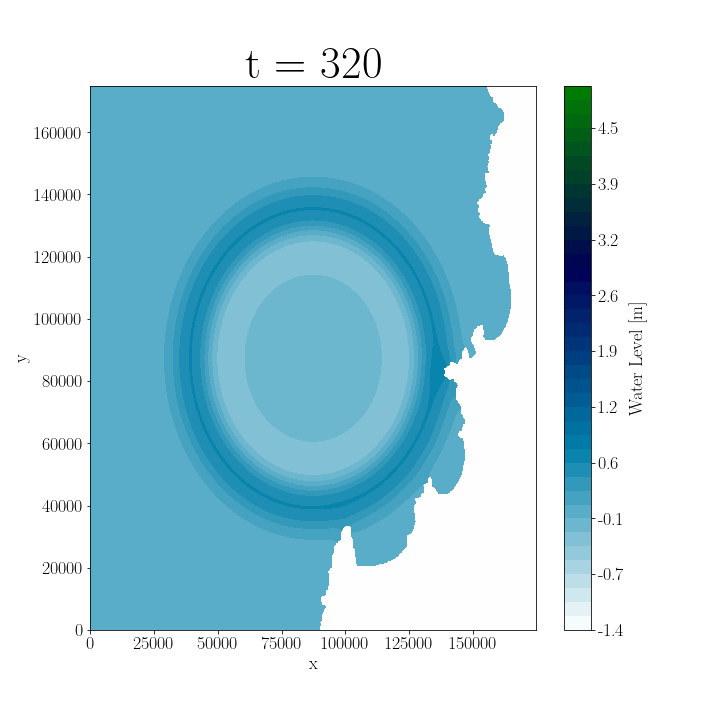
\includegraphics[width=\linewidth]{Figures/Plots/Serena3.png}
\caption{desnivel máximo = 0.71 [m]}
\end{subfigure}
\begin{subfigure}[b]{.4\linewidth}
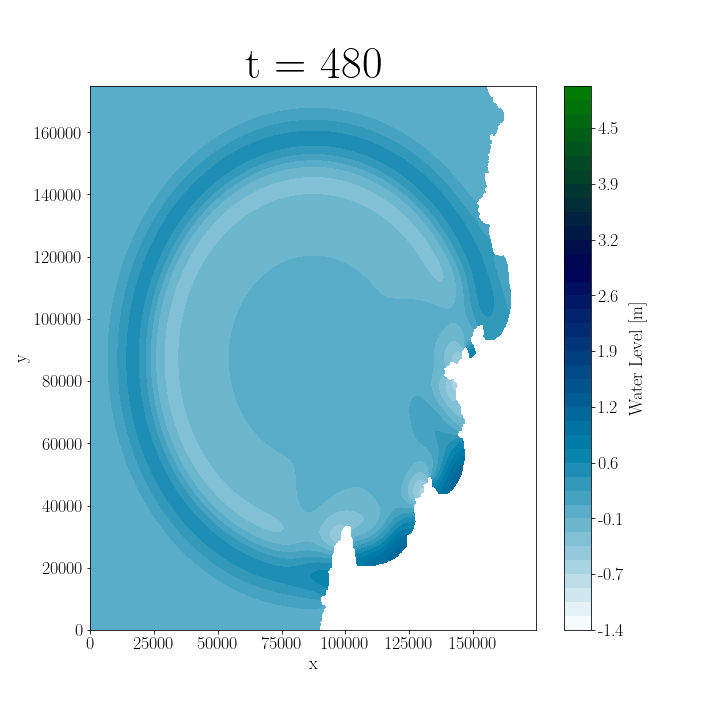
\includegraphics[width=\linewidth]{Figures/Plots/Serena4.png}
\caption{desnivel máximo = 1.17 [m]}
\end{subfigure}

\begin{subfigure}[b]{.4\linewidth}
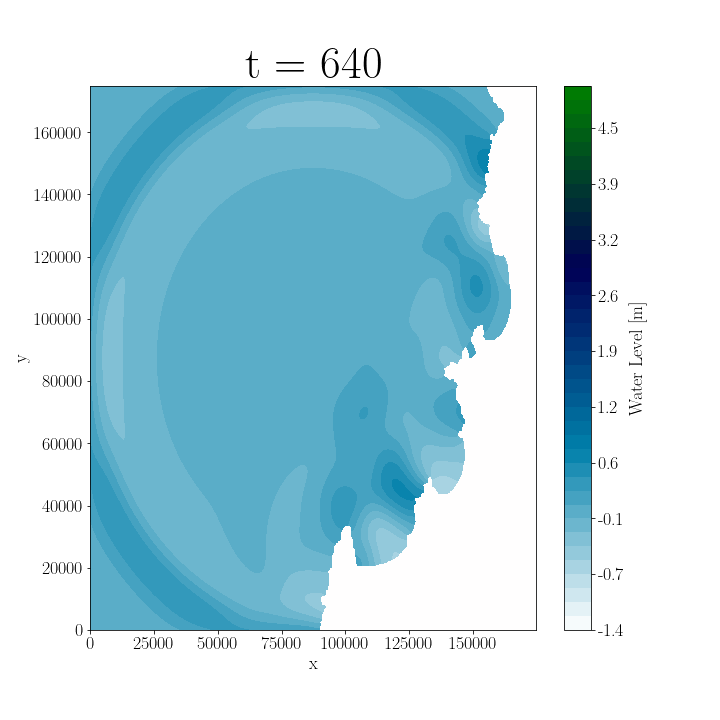
\includegraphics[width=\linewidth]{Figures/Plots/Serena5.png}
\caption{desnivel máximo = 0.70 [m]}
\end{subfigure}
\begin{subfigure}[b]{.4\linewidth}
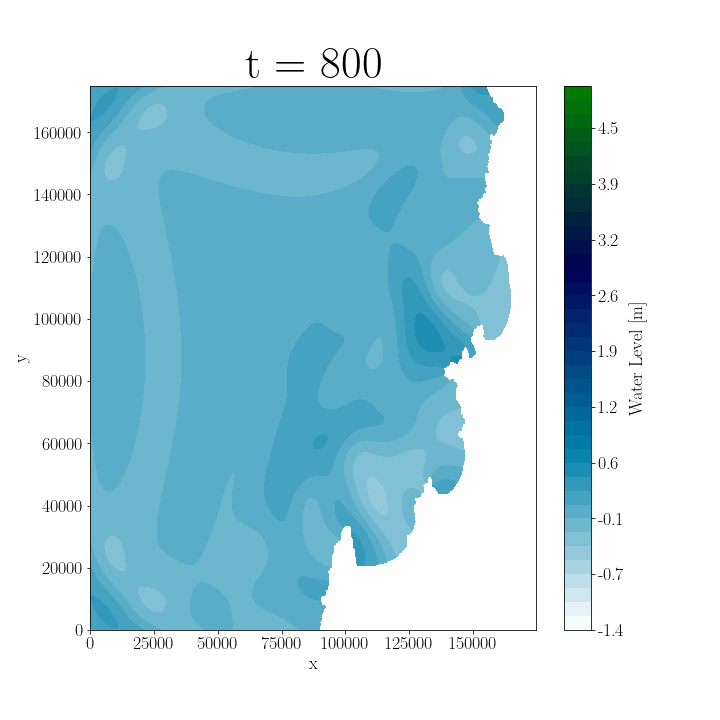
\includegraphics[width=\linewidth]{Figures/Plots/Serena6.png}
\caption{desnivel máximo = 0.50 [m]}
\end{subfigure}
\caption{Niveles de agua de la salida de ejecutar el código de LBM optimizado con el archivo de entrada \textbf{Serena}.}
\label{fig:26}
\end{figure}

%--------------------------------------------

\begin{figure}[H]
\centering
\begin{subfigure}[b]{.4\linewidth}
\includegraphics[width=\linewidth]{Figures/Plots/Valpo1.png}
\caption{desnivel máximo = 4.99 [m]}
\end{subfigure}
\begin{subfigure}[b]{.4\linewidth}
\includegraphics[width=\linewidth]{Figures/Plots/Valpo2.png}
\caption{altura máxima = 501.3 [m]}
\end{subfigure}

\begin{subfigure}[b]{.4\linewidth}
\includegraphics[width=\linewidth]{Figures/Plots/Valpo3.png}
\caption{desnivel máximo = 0.98 [m]}
\end{subfigure}
\begin{subfigure}[b]{.4\linewidth}
\includegraphics[width=\linewidth]{Figures/Plots/Valpo4.png}
\caption{desnivel máximo = 0.77 [m]}
\end{subfigure}

\begin{subfigure}[b]{.4\linewidth}
\includegraphics[width=\linewidth]{Figures/Plots/Valpo5.png}
\caption{desnivel máximo = 1.47 [m]}
\end{subfigure}
\begin{subfigure}[b]{.4\linewidth}
\includegraphics[width=\linewidth]{Figures/Plots/Valpo6.png}
\caption{desnivel máximo = 0.78 [m]}
\end{subfigure}
\caption{Niveles de agua de la salida de ejecutar el código de LBM optimizado con el archivo de entrada \textbf{Valparaiso}.}
\label{fig:27}
\end{figure}